\chapter{Código}
\section{Funciones Auxiliares}
Antes de explicar las funciones pedidas, comentaremos brevemente las funciones auxiliares que hemos utilizados
En primer lugar explicaremos algunas funciones auxiliares que hemos utilizado: 
\subsubsection{char** reservarEspacio(int)}
Esta función se encarga de reservar el espacio necesario para que nuestro array de soluciones tenga el tamaño justo, y cada elemento de dicho array pueda almacenar cualquier String que se introduzca por la entrada.
\subsubsection{void liberarEspacio(char**,int)}
Esta función se encarga de liberar la memoria dinámica tras su uso. Recibe el array de punteros donde se guarda nuestra solucion y le aplica $free$ a todos sus elementos.
\section{Función head}
La primera función a implementar es $int head(int N)$, que deberá comportarse como \textit{head(1)} y devolver las N primeras lineas en la salida estándar recibidas por entrada estándar.
En esta, primero reservamos espacio en una variable $solución$ llamando a la función $reservarEspacio$, descrita anteriormente. Luego, mediante un bucle de N iteraciones, guardamos los parámetros que vayamos recibiendo por consola en la posición i de $solución$.
Al terminar el bucle, llamamos a la función $imprimir_normal$, que lo que hará será recorrer la variable $solución$ imprimiendo por pantalla cada string guardado en cada posición del mismo.
\section{Función tail}
La segunda función a implementar es $int tail(int N)$, que deberá comportarse como \textit{tail(1)} y devolver las N últimas lineas en la salida estándar recibidas por entrada estándar.
En esta función se repite el mismo método de reservar espacio. Cuando se ha reservado espacio en la variable $solución$, se pasa a guardar la información que se pase por entrada en esta variable. Para ello, se requerirá, a parte de la variable contador i, otra variable j auxiliar, que durante el bucle se actualizará a $j=i\%n$. Esto es debido a que hay que simular que la variable solución es un array estático que hace la función de una cola. Lo hemos hecho así para no malgastar espacio de manera innecesaria, como se hubiera hecho si hubiesemos reservado un espacio determinado, y luego hubiesemos leido las N últimas posiciones (además de poder pasar por entrada tantas líneas como se desee).
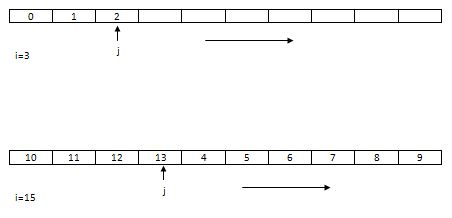
\includegraphics[width=4cm]{./img_1}
El bucle por lo tanto realiza iteraciones mientras $entrada != NULL$, y va guardando en la posición $j=i\%n$ de solución el parámetro $entrada$ recibido, y actualizando posteriormente la variable i (i++).
Por último, tras salir del bucle (CTRL+D) se procede a imprimir por pantalla el array $solución$ llamando a la función $imprimirTail$. Hemos tenido que implementar una función específica de imprimir para tail ya que esta tiene que imprimir solución empezando por una posición que no tiene por qué ser la primera.
Así, esta función imprimir recibirá como parámetros $solución$ y j (la última posición en la que se guardó el parámetro de entrada en el array) +1. Para recorrer el array, solo es necesario un bucle que vaya de i hasta N, y que en cada iteración imprima $solución[(j+i)\%N]$.
\section{Función longLines}
Por último, se nos pide implementar la función $int longlines(int N)$, que mostrará las N líneas más largas de forma ordenada recibidas por la entrada estándar.
En esta función se vuelve a utilizar el método de reservar espacio para el array $solución$. Posteriormente, entramos un bucle que iterará mientras $entrada != NULL$ en el que se irán metiendo en $solución$:
	-todas las líneas recibidas por entrada estándar si el array posee menos de N elementos
	-o en el caso de que ya esté lleno, se meterá la línea recibida si es más larga que la línea más corta del array.
Siempre que se inserte un elemento en $solución$, se hará en el sitio que corresponda, desplazando los elementos que estén a su derecha un puesto hacia la derecha (eliminando el último en el caso de que el array esté lleno)
Este proceso se lleva acabo:
	-guardando en una variable auxiliar $tam_menor$ la longitud de la línea de menor longitud insertada en el array (situada en la posición $solución[n-1]$) actualizada al principio de cada iteración,
	-una condición en la que solo entrará si se puede insertar $entrada$ en $solución$ (cuando esta es menor que la menor del array),
	-y una función auxiliar llamada $insertar$ dentro de la condición anterior que recibirá el array $solución$, la variable $entrada$ y la posición en la que ha de ser insertada, para insertarla correctamente.
La función auxiliar $insertar$, para insertar un elemento en el array recorre de derecha a izquierda hasta la posición en la que ha de insertar $entrada$, situando el elemento $solución[i-1]$ en $solución[i]$. Cuando finaliza, solo le queda por insertar en la posición correspondiente el valor entrada.
%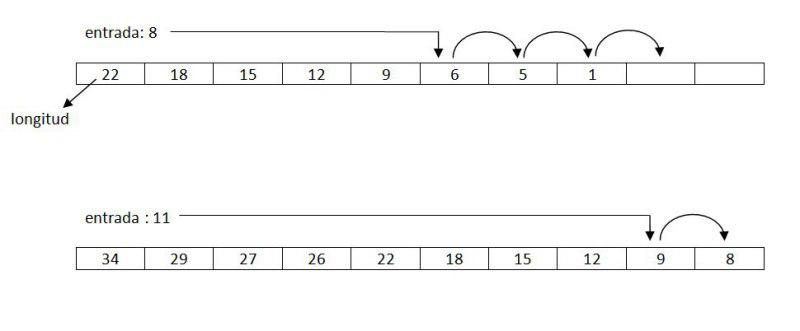
\includegraphics[width=4cm]{./img_2} -- Aun tengo que hacerla
Por último, una vez salido del bucle, solo queda imprimir por pantalla la lista solución llamando a la función $imprimir_normal$ explicada en la primera función (no es necesario crear una función imprimir específica para esta como en $tail$, puesto que el array ya viene ordenado y listo para ser impresa).
\chapter{Comentarios personales}